% Capítulo 2 - Fundamentação Teórica (versão enxuta): Aprendizado de Máquina e MLP
\section{Aprendizado de Máquina}
\label{sec:AM}

O AM estuda algoritmos que ajustam seus parâmetros a partir de exemplos, em vez de seguir regras programadas manualmente \cite{bishop2006pattern,goodfellow2016deep}. Quanto à forma de aprender, distinguem-se três paradigmas: o supervisionado, em que cada exemplo tem um rótulo conhecido e o modelo aprende a relação entre entradas e saídas; o não supervisionado, que busca estruturas em dados sem rótulo, como agrupamentos ou componentes principais \cite{jolliffe2016}; e o aprendizado por reforço, em que um agente aprende por recompensas ao interagir com um ambiente. Este trabalho trata de classificação supervisionada: cada janela de \textit{hits} recebe o rótulo da condição de operação em que foi registrada.

O objetivo do treinamento não é acertar os exemplos vistos, e sim generalizar para dados novos. A estimativa dessa capacidade depende de como os dados são separados entre treino e teste. Quando as amostras são correlacionadas no tempo ou agrupadas em unidades físicas (corridas, sessões, máquinas), uma partição aleatória coloca amostras quase idênticas nos dois conjuntos e superestima o desempenho; a validação deve então separar grupos inteiros, de modo que o teste contenha apenas unidades não vistas no treino \cite{roberts2017,varma2006}. Esse cuidado orienta os protocolos de validação descritos no Capítulo~\ref{chap:metodos}.

\section{Redes Neurais MLP}
\label{sec:MLP}

Entre os métodos de AM, as RNAs são modelos formados por unidades simples, os neurônios artificiais, que calculam uma soma ponderada das entradas seguida de uma função de ativação \cite{haykin2009neural}. A MLP é uma RNA \textit{feedforward} totalmente conectada, organizada em uma camada de entrada, uma ou mais camadas ocultas e uma camada de saída (Figura~\ref{fig:mlp}); a informação flui da entrada para a saída, sem realimentação \cite{rumelhart1986learning,haykin2009neural}.

\begin{figure}[htbp]
	\centering
	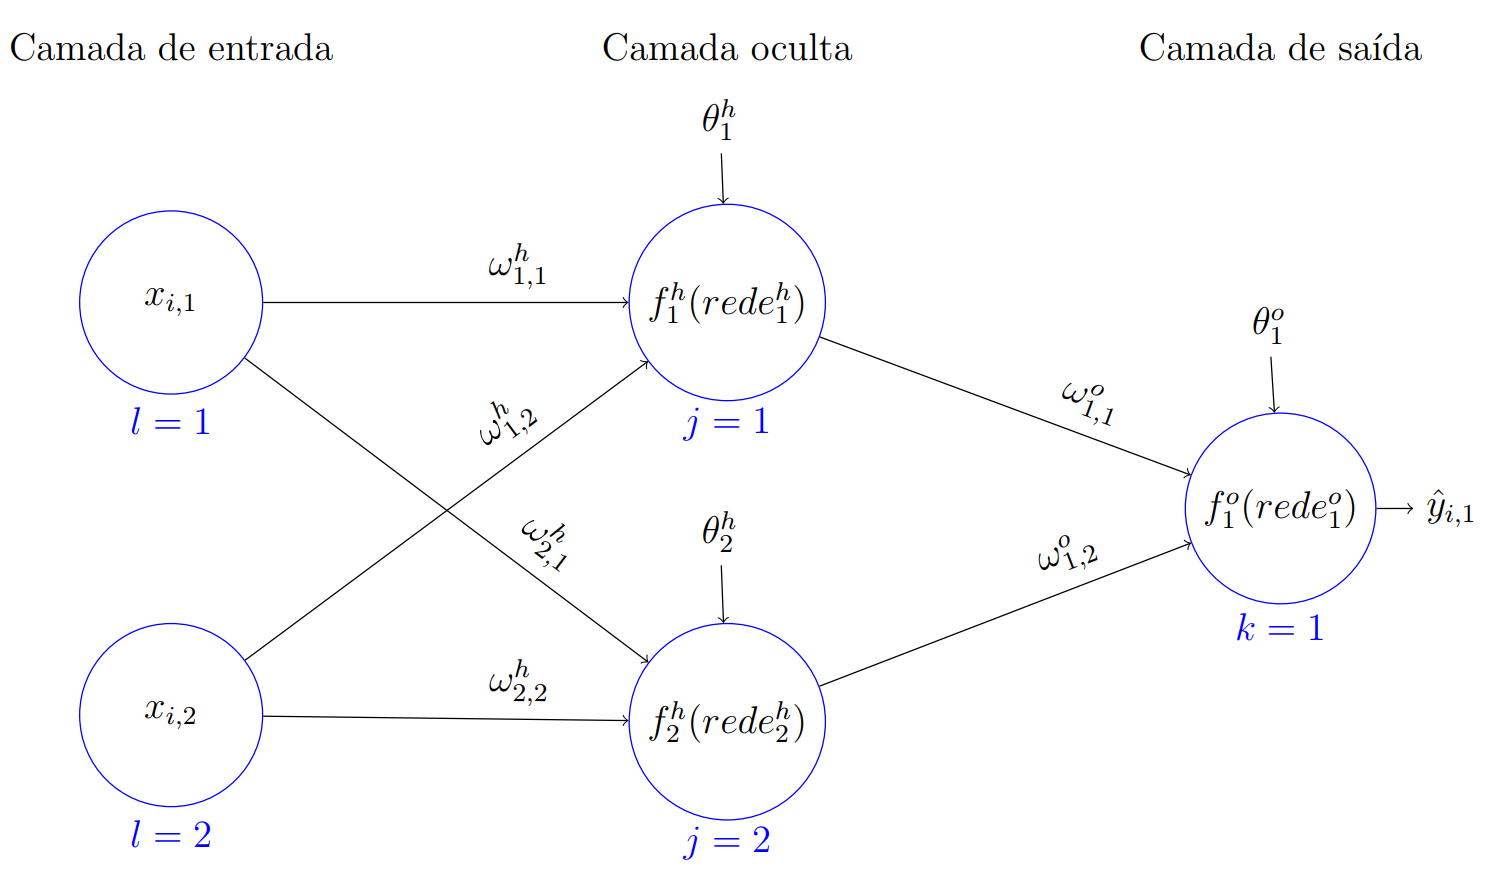
\includegraphics[width=0.8\linewidth]{figs/MLP/MLP}
	\caption{Exemplo de Perceptron Multicamadas. Fonte: o autor.}
	\label{fig:mlp}
\end{figure}

Dado um vetor de entrada \(x \in \mathbb{R}^{d}\), a MLP calcula a saída por transformações afins sucessivas, cada uma seguida de uma não linearidade:
\begin{equation}
	a^{(0)} = x,\qquad
	z^{(\ell)} = W^{(\ell)} a^{(\ell-1)} + b^{(\ell)},\qquad
	a^{(\ell)} = \phi^{(\ell)}\!\big(z^{(\ell)}\big), \quad \ell = 1,\ldots,L,
	\label{eq:mlp_forward}
\end{equation}
em que \(W^{(\ell)}\) e \(b^{(\ell)}\) são os pesos e vieses da camada \(\ell\) e \(\phi^{(\ell)}\) é a função de ativação. Nas camadas ocultas usa-se em geral a ReLU, \(\phi(z)=\max(0,z)\), que é barata de calcular e se reduz a uma comparação em \textit{hardware}. Na classificação, a camada de saída tem um neurônio por classe e a função \textit{softmax} converte os escores em probabilidades; a classe prevista é a de maior escore. É a não linearidade das camadas ocultas que permite separar classes não linearmente separáveis: uma MLP com uma única camada oculta e neurônios suficientes aproxima qualquer função contínua com precisão arbitrária \cite{cybenko1989approximation,hornik1991approximation}.

O treinamento ajusta os parâmetros \(\theta=\{(W^{(\ell)},b^{(\ell)})\}_{\ell=1}^{L}\) minimizando a perda empírica com regularização,
\begin{equation}
	\min_{\theta}\;\; \frac{1}{N}\sum_{i=1}^{N}\mathcal{L}\big(f_{\theta}(x_i),y_i\big)\;+\;\lambda\,\Omega(\theta),
	\label{eq:mlp_perda}
\end{equation}
em que \(\mathcal{L}\) é a entropia cruzada e \(\Omega(\theta)\), em geral, a norma \(\ell_2\) dos pesos. O gradiente é obtido por retropropagação (\textit{backpropagation}), que aplica a regra da cadeia às camadas da rede \cite{rumelhart1986learning}, e os parâmetros são atualizados por gradiente descendente estocástico em mini-lotes (Algoritmo~\ref{alg:mlp_sgd_minibatch}) ou por variantes adaptativas, como o Adam \cite{kingma2015adam}. A parada antecipada, que interrompe o treinamento quando o erro em um conjunto de validação deixa de cair, é outra forma usual de limitar o sobreajuste \cite{prechelt1998}.

\begin{algorithm}[htbp]
	\caption{Treinamento de uma MLP por gradiente descendente estocástico em mini-lotes}
	\label{alg:mlp_sgd_minibatch}
	\begin{algorithmic}[1]
		\Require Treino \(\mathcal{D}=\{(x_i,y_i)\}_{i=1}^{N}\); taxa \(\eta>0\); mini-lote \(B\); épocas \(E\)
		\Ensure Parâmetros treinados \(\theta\)
		\State Inicializar \(\theta\) aleatoriamente (Xavier ou He)
		\For{\(e = 1,\dots,E\)}
		\State Embaralhar \(\mathcal{D}\)
		\For{cada mini-lote \(\mathcal{B}\subset\mathcal{D}\), \(|\mathcal{B}|=B\)}
		\State Propagar \(\hat{y}=f_{\theta}(x)\) e calcular a perda \(J_{\mathcal{B}}(\theta)\)
		\State Retropropagar: \(g \gets \nabla_{\theta} J_{\mathcal{B}}(\theta)\)
		\State Atualizar: \(\theta \gets \theta - \eta g\)
		\EndFor
		\EndFor
		\State \Return \(\theta\)
	\end{algorithmic}
\end{algorithm}

Modelos mais complexos, como as redes convolucionais, superam as MLPs quando a entrada tem estrutura espacial ou sequencial explícita, mas, sobre atributos já extraídos, a MLP continua competitiva \cite{abd2023multi}. Sua inferência se reduz a produtos matriz-vetor e funções simples, com número de operações conhecido de antemão, o que favorece o mapeamento em FPGA, discutido a seguir \cite{Shawahna2019}.
